\documentclass[a4paper]{article}

% Common header definitions and settings for use in the other documentation.


% Packages
\usepackage[T1]{fontenc}    % Font Encoding
\usepackage{utopia}         % Font
%\usepackage{courier}        % Monospaced font % This messes up the code listings, as it is wider than the default.
\usepackage{titling}        % Make modifications to \maketitle
\usepackage{fancybox}       % Boxes around terminal listings.
\usepackage{fancyvrb}       % Code listings, terminal sessions, etc.
\usepackage{color}          % Define and use colours
\usepackage{tocloft}        % TOC modification
\usepackage{datetime}       % Date formatting
\usepackage{float}          % Define new float types (code)
\usepackage{caption}        % Modify caption appearance
\usepackage{todonotes}      % Add todo notes in the margin
\usepackage{framed}         % shaded environment provides background colours
\usepackage{fourier-orns}   % Ornaments around title
\usepackage{siunitx}        % Align on decimal point column type
\usepackage{ifdraft}        % Test for draft mode
\usepackage{tikz}           % Drawing Trees
\usepackage{pdflscape}      % provides landscape environment for pdflatex.
\usepackage{ifthen}         % Provides conditional tests
\usepackage{hyperref}       % Links, and nameref command




% Define some commannds for displaying the names of different things
\newcommand{\filename}[1]{\texttt{#1}}
\newcommand{\command}[1]{\texttt{#1}}
\newcommand{\var}[1]{$#1$}
\newcommand{\mathvar}[1]{#1}
\newcommand{\codefragment}[1]{\texttt{#1}}
\newcommand{\confsnippet}[1]{\texttt{#1}}

\newcommand{\class}[1]{\texttt{#1}}
\newcommand{\func}[1]{\texttt{#1}}



% Set up the appearance of todo notes
\newcommand{\todonote}[1]{\todo[backgroundcolor=white, linecolor=black, 
                                size=\small, noline]{#1}}



% Environment for showing bits of code, terminal listings, and so on.
\definecolor{box-grey}{gray}{0.4}
\newcommand{\codelabel}[1]{\textcolor{black}{#1}}
\DefineVerbatimEnvironment
    {Code}
    {Verbatim}
    {frame=single, fontsize=\scriptsize, framesep=3mm, formatcom=\vspace{7pt}, 
      xleftmargin=5mm, xrightmargin=5mm, rulecolor=\color{box-grey},
      labelposition=topline, numbersep=8pt, baselinestretch=1.2,
      numbers=left, samepage=true}
% N.B. can use option label=\codelabel{??} as needed.



% Wrapper for the above for teminal listings
% This is a pretty nasty hack, but I'm really tired. ;)
\definecolor{shadecolor}{gray}{0.95}
\setlength{\FrameSep}{-5mm}
\newenvironment{Term}
    {\begin{center}\begin{Sbox}\begin{minipage}{\linewidth-17.4mm}}
    {\end{minipage}\end{Sbox}{\setlength{\fboxsep}{3mm}\vspace*{8pt}\fcolorbox{box-grey}{shadecolor}{\TheSbox}\vspace*{6pt}}\end{center}}

\DefineVerbatimEnvironment
    {CodeTerm}
    {Verbatim}
    {frame=none, fontsize=\scriptsize, framesep=3mm, formatcom={}, 
      xleftmargin=0mm, xrightmargin=0mm, rulecolor=\color{box-grey},
      labelposition=topline, numbersep=8pt, baselinestretch=1.2,
      numbers=left, samepage=true,
      numbers=none}

% Usage:
%\begin{Code}
%\begin{CodeTerm}
%Hello, World.
%\end{CodeTerm}
%\end{Term}


% Rename the abstract
\renewcommand{\abstractname}{Introduction}



% Remove section numbering
\setcounter{secnumdepth}{0}



% Remove bold and add dots to sections in the TOC
\renewcommand\cftsecfont{\normalfont}
\renewcommand\cftsecpagefont{\normalfont}
\renewcommand{\cftsecleader}{\cftdotfill{\cftsecdotsep}}
\renewcommand\cftsecdotsep{\cftdot}
\renewcommand\cftsubsecdotsep{\cftdot}
% Show only sections in the TOC
\setcounter{tocdepth}{1}


% Configure the \maketitle command a little
\setlength{\droptitle}{-30pt}
\predate{\begin{center}\small}
\postdate{\par\end{center}}



% Set up the desired date format (20^th July 2011)
% N.B. this is very similar to the default with the 'nodayofweek' option.
\newdateformat{mydate}{\ordinaldate{\THEDAY} \monthname[\THEMONTH] \THEYEAR}
\mydate



% New float type for code listings
\floatstyle{plain}
\floatname{listing}{Listing}
\newfloat{listing}{p}{lol}



% Set up appearance of captions
\captionsetup{margin=30pt,font=small,labelfont=bf}



% Remove ugly boxes etc around hyperlinks.
\hypersetup{pdfborder = {0 0 0}}




% Tree Drawing
% {A, B, {C, D}, {E, F}}
\newcommand{\treeDrawABCDEF}{%
    \[\begin{tikzpicture}
        \node{$\{A, B\}$}
            child{node {$\{C, D\}$}}
            child{node {$\{E, F\}$}}
        ;
    \end{tikzpicture}\]
}




% Add a command to produce nice looking tildes: \urltilde
% http://stackoverflow.com/questions/718479/what-is-the-best-way-to-produce-a-tilde-in-latex-for-a-website/3900556#3900556
\catcode`~=11 % make LaTeX treat tilde (~) like a normal character
\newcommand{\urltilde}{\kern -.15em\lower .7ex\hbox{~}\kern .04em}
\catcode`~=13 % revert back to treating tilde (~) as an active character




% Allow document title to be set from main file.
\newcommand{\thedocumenttitle}{}
\newcommand{\documenttitle}[1]{%
    \renewcommand{\thedocumenttitle}{#1}
}



% Title Info
\title{Flamingo Auto-Tuning\\\decofourleft~~~\thedocumenttitle~~~\decofourright}
\author{Ben Spencer\\\normalsize\href{mailto:ben@mistymountain.co.uk}{ben@mistymountain.co.uk}}
\date{Last updated: \today}




\documenttitle{Tutorial}



\begin{document}

\maketitle

\begin{abstract}
This tutorial will lead you through a step-by-step description of setting up 
and tuning an example program. 
I'll explain each step as we go, so working through the tutorial should give 
you enough information to start tuning your own programs.
The program we'll be tuning is a blocked matrix-matrix multiplication test, 
included with the auto-tuner as an example.
If you have any comments or questions about the tuner or this tutorial then 
please feel free to get in touch.
\end{abstract}

\tableofcontents



\newpage

\section{What You'll Need}
\begin{description}
\item[The auto-tuner] \hfill\\
This is the software which performs the tuning, and is found in the 
main \filename{Autotuning} directory. The tuner can be run with the command 
\command{\urltilde{}/Autotuning/autotune} and performs a short 
self-demonstration if no arguments are provided.

\item[A program to tune] \hfill\\
This tutorial will lead you through the setup and 
tuning of a small matrix multiplication program, which is included as an 
example with the tuner. The example code can be found in the 
\filename{examples/matrix} directory. If you are going to follow along, the 
\filename{examples/matrix/original} directory contains the unmodified code, 
which we will use as a starting point. The final version of the program we end 
up with can be found in \filename{examples/matrix/modified}.

The source code for this program is shown in Listing~\ref{code:matrix_orig}.

\item[Programming tools] \hfill\\
We'll be editing and compiling the program. So you'll need a text 
editor and any program compilation tools required for your program. For this 
tutorial we'll be using \command{gcc} and \command{make} under Linux (this is 
not required by the tuner, which can tune a program using any build tools).

\end{description}


\subsection{Installing the Tuner}
To install the tuner, simply extract the .tgz file to some convenient location. 
In this tutorial, I have extracted it into my home directory, so the tuner is 
run with the command \command{\urltilde{}/Autotuning/autotune}.

You must also make sure you have Python version 2.5 or later. To check if 
Python is installed and which version you have, run the command 
\command{python -{}-version}. For more information on installing Python 
see \texttt{www.python.org}.




\clearpage

\section{What We're Aiming For}
The program calclates the product of two matrices: $C := AB$. I'm representing 
the matrices simply by a 2D array. The simplest implementation (shown below) 
processes the array \var{C} row-by-row. 
To calculate an element \var{C[i][j]}, we need to read in an entire row of 
\var{A} and an entire column of \var{B}. The speed of the program can be 
improved by increasing the re-use of any data in the fast registers or L1 
cache. 

\begin{listing}[h]
\begin{Code}
/* Perform C = C + A*B */
for(i=0; i<C_ROWS; i++)
    for(j=0; j<C_COLS; j++)
        for(k=0; k<A_COLS; k++)
            C[i][j] += A[i][k] * B[k][j];
\end{Code}

\caption{The `naive' implementation of matrix-matrix multiplication. 
This is replaced by lines~62--69 of \filename{matrix.c}}
\label{code:matrix-naive}
\end{listing}

For large matrices, row-by-row processing will not allow thr re-use of 
data from calculating \var{C[i][j]} when calculating \var{C[i][j+1]}, even 
though some of this will be the same, or at least fetched in the same cache 
lines. The idea of this program is to split the matrix into blocks and process 
one block at a time. This allows more data re-use and so the program is faster.

The block size for each loop is controlled by the parameters \var{BLOCK\_I}, 
\var{BLOCK\_J} and \var{BLOCK\_K}.
Choosing good values (that is, giving good performance) for these parameters 
would require detailed knowledge of how memory is accessed and cached on the 
machine being used. How large is the L1 cache? How long are cache lines? 

We will use the auto-tuner to automatically choose these parameter values and 
to see how much difference the choice can make to the program's performance.








\begin{listing}
\begin{Code}[label=\codelabel{matrix.c (Original Version)}]
/* 
 * Autotuning System
 * 
 * matrix.c
 * ORIGINAL VERSION
 * 
 * A simple blocked matrix-matrix multiply algorithm,
 * partitioned by the block size. This is used as an example and 
 * demonstration of the auto-tuner.
 */

#include <stdio.h>
#include <math.h>

/* Define the size of the matrices to work on. */
#define A_COLS 512
#define A_ROWS 512
#define B_COLS 512
#define B_ROWS A_COLS
#define C_COLS B_COLS
#define C_ROWS A_ROWS

/* The block size for the multiplication */
#define BLOCK_I 16
#define BLOCK_J 16
#define BLOCK_K 16


int main(void)
{
    double A[A_ROWS][A_COLS], B[B_ROWS][B_COLS], C[C_ROWS][C_COLS];
    int i, j, k, i_bl, j_bl, k_bl;
    
    printf("Blocked Matrix-Matrix Multiplication\n");
    
    /* Generate some arbitrary sample data. */
    
    for(i=0; i<A_ROWS; i++)
        for(j=0; j<A_COLS; j++)
            A[i][j] = exp(-fabs(i-j));
    
    for(i=0; i<B_ROWS; i++)
        for(j=0; j<B_COLS; j++)
            B[i][j] = exp(-fabs(i-j));
    
    
    /* Set C[][] = 0 first */
    for(i=0; i<C_ROWS; i++)
        for(j=0; j<C_COLS; j++)
            C[i][j] = 0;
    
    
\end{Code}
\end{listing}
\begin{listing}
\begin{Code}[label=\codelabel{matrix.c (Original Version, Continued)}, firstnumber=53]
    /* Blocked Multiplication: C = AB */
    /* Instead of processing an entire row of C at a time, 
     * process in small blocks of dimensions BLOCK_I * BLOCK_J. Elements 
     * required from A and B are also processed in blocks.
     * This should improve local memory reuse. */
    
    printf("(BLOCK_I = %d, BLOCK_J = %d, BLOCK_K = %d)\n", BLOCK_I, BLOCK_J, 
            BLOCK_K);
    
    
    /* Perform C = C + A*B */
    for(i=0; i<C_ROWS; i+= BLOCK_I)
        for(j=0; j<C_COLS; j+= BLOCK_J)
            for(k=0; k<A_COLS; k+= BLOCK_K)
                for(i_bl=i; i_bl<(i+BLOCK_I) && i_bl<C_ROWS; i_bl++)
                    for(j_bl=j; j_bl<(j+BLOCK_J) && j_bl<C_COLS; j_bl++)
                        for(k_bl=k; k_bl<(k+BLOCK_K) && k_bl<A_COLS; k_bl++)
                            C[i_bl][j_bl] += A[i_bl][k_bl] * B[k_bl][j_bl];
    
    /* Use C ... */
    
    return 0;
}

\end{Code}

\begin{Code}[label=\codelabel{Makefile (Original Version)}]

CC = gcc
CFLAGS = -lm

matrix: matrix.c
	$(CC) $(CFLAGS) -o matrix matrix.c

\end{Code}

\caption{The original version of \filename{matrix.c} and the 
        \filename{Makefile} used to compile it, before any modification.}
\label{code:matrix_orig}
\end{listing}






\clearpage


\section{The Build Chain}
Before tuning this program, we need to be clear about exactly what happens 
when we compile and run it. For this exampleit is fairly simple, but it is 
worth being sure of, especially when you try to tune a more complex program.

To compile the program, we run \command{make}. This reads the 
\filename{Makefile}, which in turn contains a call to \command{gcc}, which is 
run by \command{make}. \command{gcc} reads in the source file 
\filename{matrix.c} and compiles it into the executable file \filename{matrix}. 
This executable can be run with the command \command{./matrix}.




\section{Modifying The Program}
To perform the auto-tuning, the tuner will need to test various different 
settings of the parameters. So to begin with, we must modify the program a 
little to allow the parameters to be set at compile-time by the auto-tuner.


We want to tune the three block size parameters: \var{BLOCK\_I}, 
\var{BLOCK\_J} and \var{BLOCK\_K}. The first thing to do is wrap the definition 
of each in an \codefragment{\#ifndef} block, so they can be set by the 
compiler instead of being constant:
\begin{Code}[numbers=none, commandchars=\\\{\}]
\ldots
#ifndef BLOCK_I
    #define BLOCK_I 1
#endif
\ldots
\end{Code}



After this change, it is possible to set the parameters using compiler 
options. If you've made these modifications you can try it; for \command{gcc} 
the option we need is \command{-D NAME=VALUE}.
\begin{Term}
\begin{CodeTerm}[numbers=none]
$ gcc -lm -o matrix matrix.c
$ ./matrix 
Blocked Matrix-Matrix Multiplication
(BLOCK_I = 1, BLOCK_J = 1, BLOCK_K = 1)
$ gcc -lm -o matrix matrix.c -D BLOCK_I=32 -D BLOCK_J=16 -D BLOCK_K=8
$ ./matrix
Blocked Matrix-Matrix Multiplication
(BLOCK_I = 32, BLOCK_J = 16, BLOCK_K = 8)
$ 
\end{CodeTerm}
\end{Term}
%$ This stops my editor highlighting everything because it thinks we're in math mode!




We also need to modify the \filename{Makefile} so it will pass the 
parameters to the compiler. The parameters are supplied as arguments to 
\command{make} simply as \command{NAME=VALUE} pairs and can then be used 
within the \filename{Makefile} using \codefragment{\$(NAME)}. This allows us 
to supply the parameters passed to make as the \command{-D} arguments to 
\command{gcc}.
\begin{Code}[numbers=none, commandchars=\\\{\}]
gcc -o matrix matrix.c -D BLOCK_I=$(BLOCK_I) \ldots{}
\end{Code}
%$

Once this is done, we can check that the parameter values are being correctly 
passed through the build chain. The \command{-B} option forces 
\command{make} to compile, even if there has been no change to the source 
code. \command{make} usually only recompiles a file if the source code has been 
modified, but in this case only the block size parameters passed to 
\command{gcc} have been changed, so we need to force a recompilation.
\begin{Term}
\begin{CodeTerm}[numbers=none]
$ make -B BLOCK_I=3 BLOCK_J=4 BLOCK_K=5
gcc -lm -o matrix matrix.c \
					-D BLOCK_I=3 \
					-D BLOCK_J=4 \
					-D BLOCK_K=5
$ ./matrix
Blocked Matrix-Matrix Multiplication
(BLOCK_I = 3, BLOCK_J = 4, BLOCK_K = 5)
$
\end{CodeTerm}
\end{Term}
%$

The final versions of \filename{matrix.c} and the \filename{Makefile} are 
given in Listing~\ref{code:matrix-modified}.





\subsection{Aside: Make sure the test takes long enough}
%When timing tests, it is important that the running time of the relevant part 
%(in this case the multiplication) dominates the running time of the program.

We'll add a loop to the program which performs the multiplication 
multiple times. This means the running time of the program is dominated by 
the time taken by the multiplication, so the program's `overheads' will not 
add too much noise to the results. Any significant difference in the running 
time will be due to changes in the parameter values, not to random fluctuations 
in the time required to allocate memory for the arrays, and so on.
\begin{Code}[numbers=none]
...
/* For timing the test, repeat the multiplication a number of times */
#define TEST_REP 5
...
    for(rep=0; rep<TEST_REP; rep++){
        ...
    }
...
\end{Code}






\begin{listing}
\begin{Code}[label=\codelabel{matrix.c (Modified Version)}]
/* 
 * Autotuning System
 * 
 * matrix.c
 * AUTO-TUNING VERSION
 * 
 * A simple blocked matrix-matrix multiply algorithm,
 * partitioned by the block size. This is used as an example and 
 * demonstration of the auto-tuner.
 */

#include <stdio.h>
#include <math.h>

/* Define the size of the matrices to work on. */
#define A_COLS 512
#define A_ROWS 512
#define B_COLS 512
#define B_ROWS A_COLS
#define C_COLS B_COLS
#define C_ROWS A_ROWS

/* The block size for the multiplication */
#ifndef BLOCK_I
    #define BLOCK_I 1
#endif
#ifndef BLOCK_J
    #define BLOCK_J 1
#endif
#ifndef BLOCK_K
    #define BLOCK_K 1
#endif

/* For timing the test, repeat the multiplication a number of times */
#define TEST_REP 5


int main(void)
{
    double A[A_ROWS][A_COLS], B[B_ROWS][B_COLS], C[C_ROWS][C_COLS];
    int i, j, k, i_bl, j_bl, k_bl, rep;
    
    printf("Blocked Matrix-Matrix Multiplication\n");
    
    /* Generate some arbitrary sample data. */
    
    for(i=0; i<A_ROWS; i++)
        for(j=0; j<A_COLS; j++)
            A[i][j] = exp(-fabs(i-j));
    
    for(i=0; i<B_ROWS; i++)
        for(j=0; j<B_COLS; j++)
            B[i][j] = exp(-fabs(i-j));
    
    
\end{Code}
\end{listing}
\begin{listing}
\begin{Code}[label=\codelabel{Makefile (Modified Version, Continued)}, firstnumber=56]
    /* Blocked Multiplication: C = AB */
    /* Instead of processing an entire row of C at a time, 
     * process in small blocks of dimensions BLOCK_I * BLOCK_J. Elements 
     * required from A and B are also processed in blocks.
     * This should improve local memory reuse. */
    
    printf("(BLOCK_I = %d, BLOCK_J = %d, BLOCK_K = %d)\n", BLOCK_I, BLOCK_J, 
            BLOCK_K);
    for(rep=0; rep<TEST_REP; rep++){
        
        /* Set C[][] = 0 first */
        for(i=0; i<C_ROWS; i++)
            for(j=0; j<C_COLS; j++)
                C[i][j] = 0;
        
        
        /* Perform C = C + A*B */
        for(i=0; i<C_ROWS; i+= BLOCK_I)
            for(j=0; j<C_COLS; j+= BLOCK_J)
                for(k=0; k<A_COLS; k+= BLOCK_K)
                    for(i_bl=i; i_bl<(i+BLOCK_I) && i_bl<C_ROWS; i_bl++)
                        for(j_bl=j; j_bl<(j+BLOCK_J) && j_bl<C_COLS; j_bl++)
                            for(k_bl=k; k_bl<(k+BLOCK_K) && k_bl<A_COLS; k_bl++)
                                C[i_bl][j_bl] += A[i_bl][k_bl] * B[k_bl][j_bl];
        
    }
    
    /* Use C ... */
    
    return 0;
}

\end{Code}

\begin{Code}[label=\codelabel{Makefile (Modified Version)}]

CC = gcc
CFLAGS = -lm

matrix: matrix.c
	$(CC) $(CFLAGS) -o matrix matrix.c \
					-D BLOCK_I=$(BLOCK_I) \
					-D BLOCK_J=$(BLOCK_J) \
					-D BLOCK_K=$(BLOCK_K)

\end{Code}
%$
\caption{The modified versions of \filename{matrix.c} and the 
\filename{Makefile}, which are now ready for tuning.}
\label{code:matrix-modified}
\end{listing}













\clearpage

\section{Writing a Configuration File}
Now that the program and build chain is ready for auto-tuning, we must create 
a configuration file. 
This file will tell the tuner which parameters need to be tuned, what the 
possible values for them are and how to compile and run each test. 
The configuration file is simply a normal text file, similar to Linux 
configuration files, or Windows \filename{.ini} files.

The file is split into five sections: \emph{variables}, \emph{values}, 
\emph{testing}, \emph{scoring} and \emph{output}, which begin with a line 
\confsnippet{[section\_name]}. Options are set using the syntax
\confsnippet{name = value} and lines beginning with \confsnippet{\#} 
are comments. 

\textbf{All commands and paths must be given relative to the configuration 
file.}

The final configuration file is shown in Listing~\ref{code:conf-file}, and 
should be saved in the same directory as the program. A detailed description 
of all the configuration file options and their operation can be found in the 
User's Guide (\filename{doc/user.pdf}).


\subsection{The \confsnippet{[variables]} Section}
This section contains a single option, \texttt{variables}, which says which 
program parameters should be optimised. For this example we simply provide 
the list. It is possible to describe independences between the parameters 
here, which is often useful, but not for this program. Look up 
'Variable Independence' in the main User's Guide for more information on 
this.
\begin{Code}[numbers=none]
[variables]

variables = BLOCK_I, BLOCK_J, BLOCK_K
\end{Code}


\subsection{The \confsnippet{[values]} Section}
This section lists the possible values for each variable. I've chosen quite a 
wide range so I can get an idea of how blocking is ffecting the running time. 
However, don't put too many possiblities in, or the tuner will have a huge 
number of tests to run. 
Remember, as we haven't specified any independence between the variables, 
every possible combination of parameter values will be tested.
\begin{Code}[numbers=none]
[values]

BLOCK_I = 4, 8, 16, 32, 64
BLOCK_J = 4, 8, 16, 32, 64
BLOCK_K = 4, 8, 16, 32, 64
\end{Code}



\clearpage


\subsection{The \confsnippet{[testing]} Section}
This section contains the settings which define how each test is run.

The \confsnippet{compile} option sets the command used to compile each test. 
For our example, this will be a call to \command{make}, passing the parameters. 
Placeholders such as \confsnippet{\%BLOCK\_I\%} will be subsituted with the 
value of \var{BLOCK\_I} for each particular test. The substitution 
\confsnippet{\%\%ID\%\%} expands to a unique test ID, 
which is useful when more than one test might exist at once, but is not 
needed here.
\begin{Code}[numbers=none]
[testing]

compile = make -B BLOCK_I=%BLOCK_I% BLOCK_J=%BLOCK_J% BLOCK_K=%BLOCK_K%
\end{Code}

The \confsnippet{test} option gives the command required to run each test.
This command will be timed to give a score for the test.
\begin{Code}[numbers=none]
test = ./matrix
\end{Code}

The \confsnippet{clean} option can be used to run a command after a 
particular test is over (for example to remove any generated executables 
or object files), but we don't need it for our example.


\subsection{The \confsnippet{[scoring]} Section}
This section defines how tests are scored to determine which is best. 
Each test is assigned a score, which would typically be its running time, but 
any other property can be tuned.

The tuner can either minimise or maximise the score, which is chosen with the 
\confsnippet{optimal} option. The defualt is to minimise, which is what we 
want here. The possible settings are: \confsnippet{min\_time} (the default), 
\confsnippet{max\_time}, \confsnippet{min} and \confsnippet{max}. When the 
\confsnippet{min\_time} or \confsnippet{max\_time} options are used, 
the tuner will time the execution of the \confsnippet{test} command above. 

If the options \confsnippet{min} or \confsnippet{max} are used, then the 
\confsnippet{test} command must calculate its own score and output it as the 
final line of output. For this test, we want to measure the running time, but 
custom scoring is discussed in the section \emph{\nameref{sec:custom-fom}}.
%\begin{Code}[numbers=none]
%optimal = min_time
%\end{Code}


Each test can be repeated a number of times, using the \confsnippet{repeat} 
option. This helps to smooth over any variation in running time, so we'll set 
this to 3.

When a test is repeated, the overall score is some combination of the 
individual test scores. As we're measuring running time, which is only 
increased by any inaccuraccies (other programs running in the system), we 
want to choose the minimum of the individual scores as the overall score for 
each test. This is also set with the \confsnippet{repeat} option, and 
\confsnippet{min} is the default (the possible settings are: 
\confsnippet{min}, \confsnippet{max}, \confsnippet{med} or \confsnippet{avg}).
\begin{Code}[numbers=none]
repeat = 3, min

#optimal = min_time
\end{Code}



\subsection{The \confsnippet{[output]} Section}
The \confsnippet{log} option allows a log of the testing process to be 
created. If set, it gives the filename of a \filename{.csv} file which 
will list all tests performed. This log file can be used to generate graphs of 
the testing process which will help us to explore the effect that block size 
has on the program. 
We'll see how these logs can be analysed later.
\begin{Code}[numbers=none]
log = results/matrix_log.csv
\end{Code}

There is one final option, \confsnippet{script}, which allows the output of 
the tuner to be dumped into a `script' file. This reduces the amount of output 
shown on screen, so we won't use this for now.



\begin{listing}[h]
\begin{Code}[label=\codelabel{matrix\_tune.conf}]
# Autotuning System
#
# matrix_tune.conf
#
# Blocked Matrix Multiplication Tuning

[variables]

variables = BLOCK_I, BLOCK_J, BLOCK_K


[values]

BLOCK_I = 4, 8, 16, 32, 64
BLOCK_J = 4, 8, 16, 32, 64
BLOCK_K = 4, 8, 16, 32, 64


[testing]

compile = make -B BLOCK_I=%BLOCK_I% BLOCK_J=%BLOCK_J% BLOCK_K=%BLOCK_K%

test = ./matrix

#clean = 


[scoring]

repeat = 3, min

#optimal = min_time


[output]

log = results/matrix_log.csv
\end{Code}

\caption{The configuration file used for testing.}
\label{code:conf-file}
\end{listing}




\clearpage

\section{Running the Tuner}
Now that we have prepared the program and written a configuration file, we're 
ready to begin tuning. 

Before you start, it is worth making a quick calculation 
of how long the testing is likely to take. On my machine, with \var{TEST\_REP} 
set to 5(the number of repetitions of the multiplication part of the program),
running the program takes around 11s. There are 3 variables 
with 5 possible values each, so $5^3 = 125$ tests will be required. Each test 
runs the program 3 times, so the tuning will take around 70 minutes in total, 
which is fine for our tuning. If this is too long, you can reduce 
the number of possible values for the parameters, reduce the number of test 
repetitions or reduce the \var{TEST\_REP} variable within the program.

To begin testing, simply run the tuner, 
\filename{\urltilde{}/Autotuning/autotune}, with the name of 
your configuration file as an argument. This will first output what testing 
will be performed (the variables, their vales, and so on) and then begin 
running tests. This will usually take some time, but you will be able to see 
the tuner's progress on screen as it runs tests.

Once all the tests have been run, the log files will be saved 
and the tuner will tell you which setting of the parameters it found to be 
the best.
\begin{Term}
\begin{CodeTerm}[numbers=none, commandchars=+\#\@]
$ +urltilde#@/Autotuning/autotune matrix_tune.conf 

                               Autotuning System                                
                                     v0.16                                      

Retrieved settings from config file:

Variables:
BLOCK_I, BLOCK_J, BLOCK_K

Displayed as a tree:

 {BLOCK_I, BLOCK_J, BLOCK_K} 

Possible values:
BLOCK_I = ['4', '8', '16', '32', '64']
BLOCK_J = ['4', '8', '16', '32', '64']
BLOCK_K = ['4', '8', '16', '32', '64']

compile: 
make -B BLOCK_I=%BLOCK_I% BLOCK_J=%BLOCK_J% BLOCK_K=%BLOCK_K%

test: 
./matrix

Number of tests to be run: 125
(with 3 repetitions each)


Test 1:
+ldots#@
\end{CodeTerm}
\end{Term}
%$





\clearpage

\section{The Results}
Now the testing is done, it's time to look at the results. The last few lines 
of output from the tuner will tell you which parameter values resulted in the 
shortest running time. 
In this case, the optimal valuation was to set \var{BLOCK\_I} and  
\var{BLOCK\_J} to 64, and \var{BLOCK\_K} to 4.
\begin{Term}
\begin{CodeTerm}[numbers=none, commandchars=\\\{\}]
\ldots{}
Minimal valuation:
BLOCK_I = 64, BLOCK_J = 64, BLOCK_K = 4
Minimal Score:
9.95934987068
The system ran 125 tests, taking 75m47.83s.
A testing log was saved to 'matrix_log.csv'
$
\end{CodeTerm}
\end{Term}
%$

This may be useful on its own, but we can get a better understanding of how 
the parameters affect the program by looking at the log files. 
An extract from the \filename{.csv} log from my tuning is shown below.

\vspace{0.5em}
\begin{center}\tiny
    \begin{tabular}{ S[tabformat=2.0] | S[tabformat=2.0] S[tabformat=2.0] S[tabformat=2.0] | S[tabformat=2.3] S[tabformat=2.3] S[tabformat=2.3] | S[tabformat=2.3] | }
        {TestNo} & {BLOCK\_I} & {BLOCK\_K} & {BLOCK\_J} & {Score\_1} & {Score\_2} & {Score\_3} & {Score\_Overall} \\
        \hline
        1 & 4 & 4 & 4 & 12.620 & 12.647 & 13.141 & 12.620 \\
        2 & 8 & 4 & 4 & 11.237 & 11.242 & 11.585 & 11.237 \\
        3 & 16 & 4 & 4 & 11.355 & 11.362 & 11.533 & 11.355 \\
        4 & 32 & 4 & 4 & 11.107 & 11.293 & 11.341 & 11.107 \\
        5 & 64 & 4 & 4 & 10.805 & 11.086 & 11.207 & 10.805 \\
        6 & 4 & 8 & 4 & 12.140 & 12.188 & 12.830 & 12.140 \\
        7 & 8 & 8 & 4 & 11.541 & 11.556 & 11.581 & 11.541 \\
        \multicolumn{1}{c|}{\vdots} & \multicolumn{3}{c|}{\vdots} & \multicolumn{3}{c|}{\vdots} & \multicolumn{1}{c|}{\vdots} \\[5pt]
        124 & 32 & 64 & 64 & 12.921 & 12.936 & 12.961 & 12.921 \\
        125 & 64 & 64 & 64 & 12.873 & 12.879 & 12.924 & 12.873 \\
        \hline
    \end{tabular}
\end{center}
\vspace{0.3em}

To produce a graph of the testing results, we use one of the tuner's 
output utilities to convert the \filename{.csv} log into a \command{gnuplot} 
\filename{.plt} script. This \filename{.plt} file can be edited by hand to 
alter the appearance of the graph, for example to change the labels or colours.
Then we can use the \command{gnuplot} plotting program to generate the graph. 
Some instructions are given at the top of the generated 
\filename{.plt} file, and here is what I did. The graph I generated is shown 
on Page~\pageref{fig:tuning-results-graph}. 
For more information on \command{gnuplot}, see \texttt{www.gnuplot.info}.
\begin{Term}
\begin{CodeTerm}[numbers=none, commandchars=\\\{\}]
$ \urltilde{}/Autotuning/utilities/output_gnuplot.py matrix_log.csv matrix_log.plt
Reading 'matrix_log.csv'
Generating gnuplot script
Writing 'matrix_plot.plt'
Done
There are some instructions for generating a png at the top of the file.
$ gnuplot
\ldots{}
gnuplot> set terminal png large size 1500, 1800
Terminal type set to 'png'
Options are 'nocrop font /usr/share/fonts/truetype/ttf-liberation/LiberationSans
-Regular.ttf 14 size 1500,1800 '
gnuplot> set output './matrix_plot.png'
gnuplot> load './matrix_plot.plt'
gnuplot> exit
$
\end{CodeTerm}
\end{Term}
%$







\begin{landscape}
\begin{figure}[p]
\begin{center}
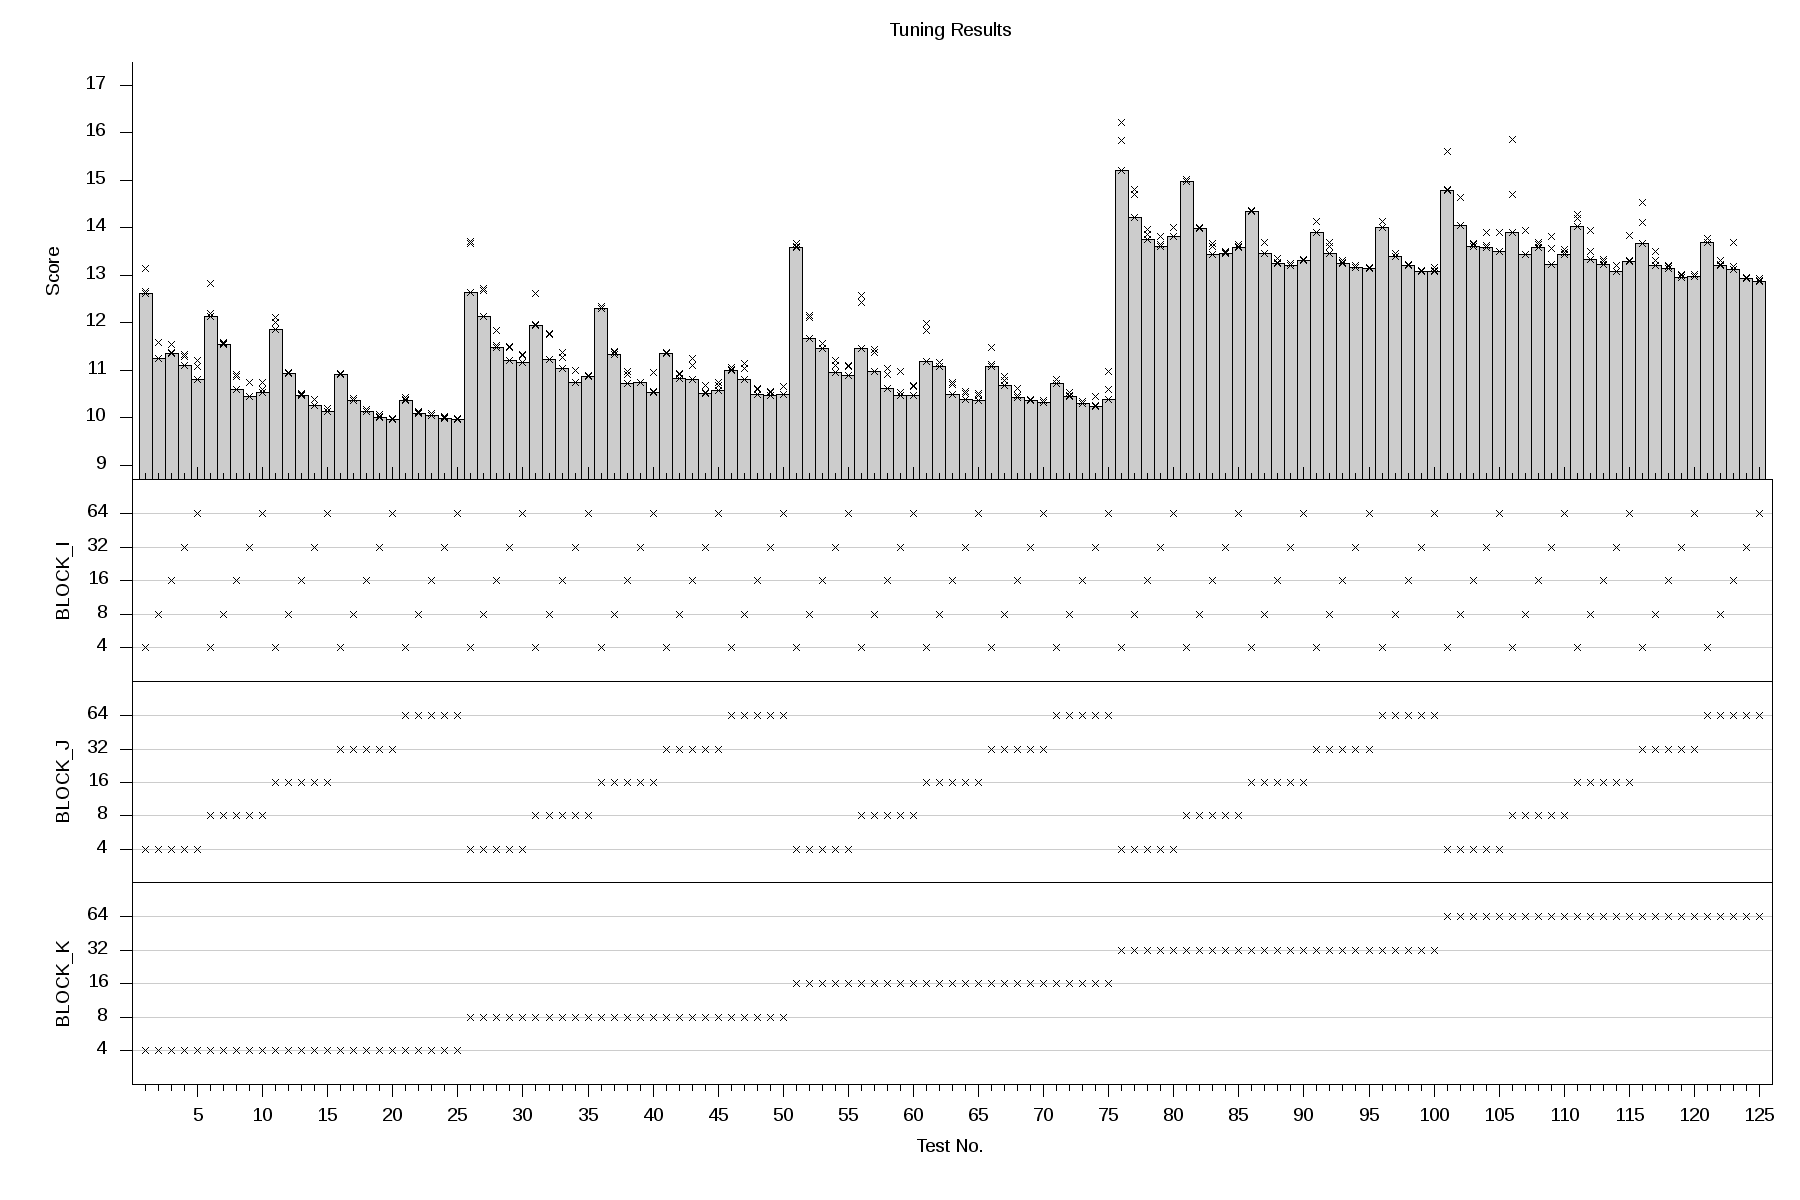
\includegraphics[height=12cm]{tutorial_files/matrix_plot.png}
\caption{The graph of testing results, generated by \command{gnuplot} using 
\filename{matrix\_plot.plt}}
\label{fig:tuning-results-graph}
\end{center}
\end{figure}
\end{landscape}







\subsection{Analysis}
The bottom half of the graph shows which tests were run. The test number is 
shown along the x-axis, and the setting of each variable is shown on the 
subgraphs. The top half of the graph shows the score for 
each test. The grey bars show the overall score which is used to compare the 
tests, and the small crosses show the individual scores from each repetition 
of the test.

The patterns in the graph allow us to clearly see how each variable affects 
performace. Firstly, the graph has five distinct `sections' or `steps', 
which corrspond to the changing values of \var{BLOCK\_K}. It seems 
that 4, 8 and 16 were all quite good values, while 32 and 64 were 
significantly worse. Next, we can see a `saw-tooth' pattern within each 
section. These correspond to the settings of \var{BLOCK\_J} and seem to 
decrease as \var{BLOCK\_J} increases, indicating that high values are better.
Finally, each peak and dip of the saw-tooth pattern corresponds to varying 
\var{BLOCK\_I}. Higher values of \var{BLOCK\_I} also seem to be best.

%Looking at the graph allows us to see that the optimal valuation will 
%porobably be $\mathvar{BLOCK\_I} = 64, \mathvar{BLOCK\_J} = 64, \mathvar{BLOCK\_K} = 4$.
%This can be read off the graph even if there were an anomalous result which 
%actually led the system to choose a different valuation. In this case, 
%the tuner chose exactly this valuation.







\subsection{Further Tuning}
The optimal results of both \var{BLOCK\_I} and \var{BLOCK\_J} were at the upper 
extreme of the possible values we supplied. Also, there is a definite trend 
towards higher values of these two variables being better. This could 
motivate the idea to try another tuning run, but with even higher values of 
\var{BLOCK\_I} and \var{BLOCK\_J}. For \var{BLOCK\_K}, we might choose to tune 
a lower range of values, or we might choose a wider, sparser range, to cover 
more possiblities both higher and lower.

This type of additional run allows us to perform very detailed tuning, 
but only on a very small part of the space of possible values. If we had 
tried to perform the detailed tuning in the first place, there would have 
been far too many tests. A coarse tuning gives enough information to 
intelligently choose a more refined search.


\clearpage

\section{Using a Custom Figure-of-Merit}
\label{sec:custom-fom}
The testing we performed timed the entire running of the program and used 
this as the score for a test. In some cases, you will want to use some other 
measurement as the score for a test. In our example, if we decided that the 
program overheads were large compared to the part we wanted to time, we could 
use a timer of only the multiplication part to provide the score.

To set this up, we would add timing code to our program, which timed only the 
multiplication. In the configuration file, instead of using the 
option \confsnippet{optimal~=~min\_time}, we would use 
\confsnippet{optimal~=~min}. This tells the tuner that you are going to 
provide the score yourself, so it will not time the entire execution. 
Instead, it will expect the score to be given as the last line of output of 
the test. So for our example, we would print out the time taken by the 
multiplication as the last piece of output from the program. The tuner would 
then read this and use it as a score.

When using a custom figure-of-merit like this, you are not 
restricted to using running time at all. If you wanted to optimise the memory 
bandwidth, or some other property, all you need to do is have your program 
measure it, then output the score (as a float or integer) as the last line 
of output.

The User's Guide contains more information about using a custom 
figure-of-merit to tune other properties of a program than the overall 
running time.




\section{The End}
Hopefully this tutorial has shown you enough to let you begin tuning your own 
programs. The main takeaway is to see how the tuning process works: first 
modifying the program and build chain, then setting up a configuration file, 
and finally running the tuner. It is important to be clear about how the 
variables from the tuner will be passed from the tuner to the 
\filename{Makefile}, then to \command{gcc} and finally to the program.

I have covered all but one of the program's main features. I have not 
discussed Variable Independence at all, which allows you to reduce the 
number of tests which need to be run. For more complex programs, 
the savings in tuning time can be substantial.

For more information about the tuner and a more detailed description of each 
option, you can look at the User's Guide (\filename{doc/user.pdf}). 
Alternatively, try some of the other example programs included with the tuner 
(found in \filename{examples/}).

If you have any comments or questions on the tuner or this tutorial, please 
feel free to get in touch.





\end{document}
